\documentclass[twoside]{book}

% Packages required by doxygen
\usepackage{fixltx2e}
\usepackage{calc}
\usepackage{doxygen}
\usepackage{graphicx}
\usepackage[utf8]{inputenc}
\usepackage{makeidx}
\usepackage{multicol}
\usepackage{multirow}
\PassOptionsToPackage{warn}{textcomp}
\usepackage{textcomp}
\usepackage[nointegrals]{wasysym}
\usepackage[table]{xcolor}

% Font selection
\usepackage[T1]{fontenc}
\usepackage{mathptmx}
\usepackage[scaled=.90]{helvet}
\usepackage{courier}
\usepackage{amssymb}
\usepackage{sectsty}
\renewcommand{\familydefault}{\sfdefault}
\allsectionsfont{%
  \fontseries{bc}\selectfont%
  \color{darkgray}%
}
\renewcommand{\DoxyLabelFont}{%
  \fontseries{bc}\selectfont%
  \color{darkgray}%
}
\newcommand{\+}{\discretionary{\mbox{\scriptsize$\hookleftarrow$}}{}{}}

% Page & text layout
\usepackage{geometry}
\geometry{%
  a4paper,%
  top=2.5cm,%
  bottom=2.5cm,%
  left=2.5cm,%
  right=2.5cm%
}
\tolerance=750
\hfuzz=15pt
\hbadness=750
\setlength{\emergencystretch}{15pt}
\setlength{\parindent}{0cm}
\setlength{\parskip}{0.2cm}
\makeatletter
\renewcommand{\paragraph}{%
  \@startsection{paragraph}{4}{0ex}{-1.0ex}{1.0ex}{%
    \normalfont\normalsize\bfseries\SS@parafont%
  }%
}
\renewcommand{\subparagraph}{%
  \@startsection{subparagraph}{5}{0ex}{-1.0ex}{1.0ex}{%
    \normalfont\normalsize\bfseries\SS@subparafont%
  }%
}
\makeatother

% Headers & footers
\usepackage{fancyhdr}
\pagestyle{fancyplain}
\fancyhead[LE]{\fancyplain{}{\bfseries\thepage}}
\fancyhead[CE]{\fancyplain{}{}}
\fancyhead[RE]{\fancyplain{}{\bfseries\leftmark}}
\fancyhead[LO]{\fancyplain{}{\bfseries\rightmark}}
\fancyhead[CO]{\fancyplain{}{}}
\fancyhead[RO]{\fancyplain{}{\bfseries\thepage}}
\fancyfoot[LE]{\fancyplain{}{}}
\fancyfoot[CE]{\fancyplain{}{}}
\fancyfoot[RE]{\fancyplain{}{\bfseries\scriptsize Generated on Sun Nov 9 2014 11\+:47\+:38 for S\+W\+E1\+D by Doxygen }}
\fancyfoot[LO]{\fancyplain{}{\bfseries\scriptsize Generated on Sun Nov 9 2014 11\+:47\+:38 for S\+W\+E1\+D by Doxygen }}
\fancyfoot[CO]{\fancyplain{}{}}
\fancyfoot[RO]{\fancyplain{}{}}
\renewcommand{\footrulewidth}{0.4pt}
\renewcommand{\chaptermark}[1]{%
  \markboth{#1}{}%
}
\renewcommand{\sectionmark}[1]{%
  \markright{\thesection\ #1}%
}

% Indices & bibliography
\usepackage{natbib}
\usepackage[titles]{tocloft}
\setcounter{tocdepth}{3}
\setcounter{secnumdepth}{5}
\makeindex

% Hyperlinks (required, but should be loaded last)
\usepackage{ifpdf}
\ifpdf
  \usepackage[pdftex,pagebackref=true]{hyperref}
\else
  \usepackage[ps2pdf,pagebackref=true]{hyperref}
\fi
\hypersetup{%
  colorlinks=true,%
  linkcolor=blue,%
  citecolor=blue,%
  unicode%
}

% Custom commands
\newcommand{\clearemptydoublepage}{%
  \newpage{\pagestyle{empty}\cleardoublepage}%
}


%===== C O N T E N T S =====

\begin{document}

% Titlepage & ToC
\hypersetup{pageanchor=false,
             bookmarks=true,
             bookmarksnumbered=true,
             pdfencoding=unicode
            }
\pagenumbering{roman}
\begin{titlepage}
\vspace*{7cm}
\begin{center}%
{\Large S\+W\+E1\+D }\\
\vspace*{1cm}
{\large Generated by Doxygen 1.8.8}\\
\vspace*{0.5cm}
{\small Sun Nov 9 2014 11:47:38}\\
\end{center}
\end{titlepage}
\clearemptydoublepage
\tableofcontents
\clearemptydoublepage
\pagenumbering{arabic}
\hypersetup{pageanchor=true}

%--- Begin generated contents ---
\chapter{Namespace Index}
\section{Namespace List}
Here is a list of all namespaces with brief descriptions\+:\begin{DoxyCompactList}
\item\contentsline{section}{\hyperlink{namespacesolver}{solver} }{\pageref{namespacesolver}}{}
\end{DoxyCompactList}

\chapter{Hierarchical Index}
\section{Class Hierarchy}
This inheritance list is sorted roughly, but not completely, alphabetically\+:\begin{DoxyCompactList}
\item \contentsline{section}{solver\+:\+:F\+Wave$<$ T $>$}{\pageref{classsolver_1_1FWave}}{}
\item \contentsline{section}{solver\+:\+:F\+Wave$<$ T $>$\+:\+:Quantity}{\pageref{structsolver_1_1FWave_1_1Quantity}}{}
\item Test\+Suite\begin{DoxyCompactList}
\item \contentsline{section}{F\+Wave\+Test}{\pageref{classFWaveTest}}{}
\end{DoxyCompactList}
\end{DoxyCompactList}

\chapter{Class Index}
\section{Class List}
Here are the classes, structs, unions and interfaces with brief descriptions\+:\begin{DoxyCompactList}
\item\contentsline{section}{\hyperlink{classsolver_1_1FWave}{solver\+::\+F\+Wave$<$ T $>$} }{\pageref{classsolver_1_1FWave}}{}
\item\contentsline{section}{\hyperlink{classFWaveTest}{F\+Wave\+Test} }{\pageref{classFWaveTest}}{}
\item\contentsline{section}{\hyperlink{structsolver_1_1FWave_1_1Quantity}{solver\+::\+F\+Wave$<$ T $>$\+::\+Quantity} }{\pageref{structsolver_1_1FWave_1_1Quantity}}{}
\end{DoxyCompactList}

\chapter{File Index}
\section{File List}
Here is a list of all files with brief descriptions\+:\begin{DoxyCompactList}
\item\contentsline{section}{\hyperlink{FWave_8hpp}{F\+Wave.\+hpp} }{\pageref{FWave_8hpp}}{}
\item\contentsline{section}{\hyperlink{FWaveTest_8h}{F\+Wave\+Test.\+h} }{\pageref{FWaveTest_8h}}{}
\end{DoxyCompactList}

\chapter{Namespace Documentation}
\hypertarget{namespacesolver}{}\section{solver Namespace Reference}
\label{namespacesolver}\index{solver@{solver}}
\subsection*{Classes}
\begin{DoxyCompactItemize}
\item 
class \hyperlink{classsolver_1_1FWave}{F\+Wave}
\end{DoxyCompactItemize}

\chapter{Class Documentation}
\hypertarget{classsolver_1_1FWave}{}\section{solver\+:\+:F\+Wave$<$ T $>$ Class Template Reference}
\label{classsolver_1_1FWave}\index{solver\+::\+F\+Wave$<$ T $>$@{solver\+::\+F\+Wave$<$ T $>$}}


{\ttfamily \#include $<$F\+Wave.\+hpp$>$}

\subsection*{Classes}
\begin{DoxyCompactItemize}
\item 
struct \hyperlink{structsolver_1_1FWave_1_1Quantity}{Quantity}
\end{DoxyCompactItemize}
\subsection*{Public Types}
\begin{DoxyCompactItemize}
\item 
enum \hyperlink{classsolver_1_1FWave_a311594734127c119adecdc164293b705}{Cell\+Type} \{ \hyperlink{classsolver_1_1FWave_a311594734127c119adecdc164293b705a06547946a0e672670e8462b6ba2dea09}{Wet\+Wet}, 
\hyperlink{classsolver_1_1FWave_a311594734127c119adecdc164293b705a5801fb68072c39ed9cabdf7e8fe3aec9}{Dry\+Dry}, 
\hyperlink{classsolver_1_1FWave_a311594734127c119adecdc164293b705a87b36bf7ab4331cb5246dccc030afa77}{Wet\+Dry}, 
\hyperlink{classsolver_1_1FWave_a311594734127c119adecdc164293b705a94f242a5ccfed3c65930b2d4bd7781dc}{Dry\+Wet}
 \}
\end{DoxyCompactItemize}
\subsection*{Public Member Functions}
\begin{DoxyCompactItemize}
\item 
\hyperlink{classsolver_1_1FWave_a446e2721d799afa5612a3a2b8c30d668}{F\+Wave} ()
\item 
void \hyperlink{classsolver_1_1FWave_adfb0c6a6e5e0de65210e3f4b137582ee}{compute\+Net\+Updates} (T hl, T hr, T hul, T hur, T bl, T br, T \&outhl, T \&outhr, T \&outhul, T \&outhur, T \&outmax\+W\+S)
\end{DoxyCompactItemize}
\subsection*{Static Public Attributes}
\begin{DoxyCompactItemize}
\item 
static const T \hyperlink{classsolver_1_1FWave_ac3884c16c1822530961884e9f52304a2}{g} = 9.\+81
\item 
static const T \hyperlink{classsolver_1_1FWave_aa7adb43b1b39a0f78d0784e05f7b040e}{zero\+Tol} = 0.\+0000001
\item 
static const T \hyperlink{classsolver_1_1FWave_a81a9f987fa6f23ec96c557615cee17f5}{dry\+Tol} = 0.\+01
\end{DoxyCompactItemize}
\subsection*{Private Member Functions}
\begin{DoxyCompactItemize}
\item 
\hyperlink{classsolver_1_1FWave_a311594734127c119adecdc164293b705}{Cell\+Type} \hyperlink{classsolver_1_1FWave_a96e9fc19889c093a3b566e84165574f7}{compute\+Boundary} (\hyperlink{structsolver_1_1FWave_1_1Quantity}{Quantity} \&ql, \hyperlink{structsolver_1_1FWave_1_1Quantity}{Quantity} \&qr, T $\ast$bl, T $\ast$br)
\item 
T \hyperlink{classsolver_1_1FWave_afff9d749891aaa8e6efcf66962549d08}{compute\+Height\+Roe} (\hyperlink{structsolver_1_1FWave_1_1Quantity}{Quantity} \&ql, \hyperlink{structsolver_1_1FWave_1_1Quantity}{Quantity} \&qr)
\item 
T \hyperlink{classsolver_1_1FWave_a70acc5f433ed8236e5258fdb612c143a}{compute\+Velo\+Roe} (\hyperlink{structsolver_1_1FWave_1_1Quantity}{Quantity} \&ql, \hyperlink{structsolver_1_1FWave_1_1Quantity}{Quantity} \&qr)
\item 
void \hyperlink{classsolver_1_1FWave_ad17bab0aaaf1cead99aaae8df2d1207a}{compute\+Eigencoeff} (\hyperlink{structsolver_1_1FWave_1_1Quantity}{Quantity} \&ql, \hyperlink{structsolver_1_1FWave_1_1Quantity}{Quantity} \&qr, T lambda1, T lambda2, T br, T bl, T out\mbox{[}2\mbox{]})
\item 
void \hyperlink{classsolver_1_1FWave_a69befe04e701c375627d32b608032dae}{flux} (\hyperlink{structsolver_1_1FWave_1_1Quantity}{Quantity} \&q, T out\mbox{[}2\mbox{]})
\item 
void \hyperlink{classsolver_1_1FWave_ad9de808829e9fdfb2d299643cc53448b}{inverse\+Matrix} (T m\mbox{[}2\mbox{]}\mbox{[}2\mbox{]})
\item 
void \hyperlink{classsolver_1_1FWave_a00283d0def2919fea709631aca3e583a}{compute\+Wave\+Z} (T ec, T lambda, T out\mbox{[}2\mbox{]})
\end{DoxyCompactItemize}


\subsection{Member Enumeration Documentation}
\hypertarget{classsolver_1_1FWave_a311594734127c119adecdc164293b705}{}\index{solver\+::\+F\+Wave@{solver\+::\+F\+Wave}!Cell\+Type@{Cell\+Type}}
\index{Cell\+Type@{Cell\+Type}!solver\+::\+F\+Wave@{solver\+::\+F\+Wave}}
\subsubsection[{Cell\+Type}]{\setlength{\rightskip}{0pt plus 5cm}template$<$typename T$>$ enum {\bf solver\+::\+F\+Wave\+::\+Cell\+Type}}\label{classsolver_1_1FWave_a311594734127c119adecdc164293b705}
\begin{Desc}
\item[Enumerator]\par
\begin{description}
\index{Wet\+Wet@{Wet\+Wet}!solver\+::\+F\+Wave@{solver\+::\+F\+Wave}}\index{solver\+::\+F\+Wave@{solver\+::\+F\+Wave}!Wet\+Wet@{Wet\+Wet}}\item[{\em 
\hypertarget{classsolver_1_1FWave_a311594734127c119adecdc164293b705a06547946a0e672670e8462b6ba2dea09}{}Wet\+Wet\label{classsolver_1_1FWave_a311594734127c119adecdc164293b705a06547946a0e672670e8462b6ba2dea09}
}]Both cells are wet \index{Dry\+Dry@{Dry\+Dry}!solver\+::\+F\+Wave@{solver\+::\+F\+Wave}}\index{solver\+::\+F\+Wave@{solver\+::\+F\+Wave}!Dry\+Dry@{Dry\+Dry}}\item[{\em 
\hypertarget{classsolver_1_1FWave_a311594734127c119adecdc164293b705a5801fb68072c39ed9cabdf7e8fe3aec9}{}Dry\+Dry\label{classsolver_1_1FWave_a311594734127c119adecdc164293b705a5801fb68072c39ed9cabdf7e8fe3aec9}
}]Both cells are dry \index{Wet\+Dry@{Wet\+Dry}!solver\+::\+F\+Wave@{solver\+::\+F\+Wave}}\index{solver\+::\+F\+Wave@{solver\+::\+F\+Wave}!Wet\+Dry@{Wet\+Dry}}\item[{\em 
\hypertarget{classsolver_1_1FWave_a311594734127c119adecdc164293b705a87b36bf7ab4331cb5246dccc030afa77}{}Wet\+Dry\label{classsolver_1_1FWave_a311594734127c119adecdc164293b705a87b36bf7ab4331cb5246dccc030afa77}
}]The left cell is wet, the right cell is dry \index{Dry\+Wet@{Dry\+Wet}!solver\+::\+F\+Wave@{solver\+::\+F\+Wave}}\index{solver\+::\+F\+Wave@{solver\+::\+F\+Wave}!Dry\+Wet@{Dry\+Wet}}\item[{\em 
\hypertarget{classsolver_1_1FWave_a311594734127c119adecdc164293b705a94f242a5ccfed3c65930b2d4bd7781dc}{}Dry\+Wet\label{classsolver_1_1FWave_a311594734127c119adecdc164293b705a94f242a5ccfed3c65930b2d4bd7781dc}
}]The left cell is dry, the right cell is wet \end{description}
\end{Desc}


\subsection{Constructor \& Destructor Documentation}
\hypertarget{classsolver_1_1FWave_a446e2721d799afa5612a3a2b8c30d668}{}\index{solver\+::\+F\+Wave@{solver\+::\+F\+Wave}!F\+Wave@{F\+Wave}}
\index{F\+Wave@{F\+Wave}!solver\+::\+F\+Wave@{solver\+::\+F\+Wave}}
\subsubsection[{F\+Wave}]{\setlength{\rightskip}{0pt plus 5cm}template$<$typename T$>$ {\bf solver\+::\+F\+Wave}$<$ T $>$\+::{\bf F\+Wave} (
\begin{DoxyParamCaption}
{}
\end{DoxyParamCaption}
)\hspace{0.3cm}{\ttfamily [inline]}}\label{classsolver_1_1FWave_a446e2721d799afa5612a3a2b8c30d668}


\subsection{Member Function Documentation}
\hypertarget{classsolver_1_1FWave_a96e9fc19889c093a3b566e84165574f7}{}\index{solver\+::\+F\+Wave@{solver\+::\+F\+Wave}!compute\+Boundary@{compute\+Boundary}}
\index{compute\+Boundary@{compute\+Boundary}!solver\+::\+F\+Wave@{solver\+::\+F\+Wave}}
\subsubsection[{compute\+Boundary}]{\setlength{\rightskip}{0pt plus 5cm}template$<$typename T$>$ {\bf Cell\+Type} {\bf solver\+::\+F\+Wave}$<$ T $>$\+::compute\+Boundary (
\begin{DoxyParamCaption}
\item[{{\bf Quantity} \&}]{ql, }
\item[{{\bf Quantity} \&}]{qr, }
\item[{T $\ast$}]{bl, }
\item[{T $\ast$}]{br}
\end{DoxyParamCaption}
)\hspace{0.3cm}{\ttfamily [inline]}, {\ttfamily [private]}}\label{classsolver_1_1FWave_a96e9fc19889c093a3b566e84165574f7}
Look up the height of both sides and determine the property of the edge as celltype.


\begin{DoxyParams}{Parameters}
{\em \&ql} & \hyperlink{structsolver_1_1FWave_1_1Quantity}{Quantity} \mbox{[}h, (hu)T\mbox{]} of left cell \\
\hline
{\em \&qr} & \hyperlink{structsolver_1_1FWave_1_1Quantity}{Quantity} \mbox{[}h, (hu)T\mbox{]} of right cell \\
\hline
\end{DoxyParams}
\begin{DoxyReturn}{Returns}
Cell\+Type state of the edge 
\end{DoxyReturn}
\hypertarget{classsolver_1_1FWave_ad17bab0aaaf1cead99aaae8df2d1207a}{}\index{solver\+::\+F\+Wave@{solver\+::\+F\+Wave}!compute\+Eigencoeff@{compute\+Eigencoeff}}
\index{compute\+Eigencoeff@{compute\+Eigencoeff}!solver\+::\+F\+Wave@{solver\+::\+F\+Wave}}
\subsubsection[{compute\+Eigencoeff}]{\setlength{\rightskip}{0pt plus 5cm}template$<$typename T$>$ void {\bf solver\+::\+F\+Wave}$<$ T $>$\+::compute\+Eigencoeff (
\begin{DoxyParamCaption}
\item[{{\bf Quantity} \&}]{ql, }
\item[{{\bf Quantity} \&}]{qr, }
\item[{T}]{lambda1, }
\item[{T}]{lambda2, }
\item[{T}]{br, }
\item[{T}]{bl, }
\item[{T}]{out\mbox{[}2\mbox{]}}
\end{DoxyParamCaption}
)\hspace{0.3cm}{\ttfamily [inline]}, {\ttfamily [private]}}\label{classsolver_1_1FWave_ad17bab0aaaf1cead99aaae8df2d1207a}
Compute the eigencoefficients a\+\_\+p by using the wavespeeds and the flux formula. (Formula (8))


\begin{DoxyParams}{Parameters}
{\em \&ql} & \hyperlink{structsolver_1_1FWave_1_1Quantity}{Quantity} \mbox{[}h, (hu)T\mbox{]} of left cell \\
\hline
{\em \&qr} & \hyperlink{structsolver_1_1FWave_1_1Quantity}{Quantity} \mbox{[}h, (hu)T\mbox{]} of right cell \\
\hline
{\em lambda1} & Wavespeed 1 \\
\hline
{\em lambda2} & Wavespeed 2 \\
\hline
{\em out\mbox{[}2\mbox{]}} & output array of size 2, contains eigencoefficients a\+\_\+1 and a\+\_\+2 \\
\hline
\end{DoxyParams}
\hypertarget{classsolver_1_1FWave_afff9d749891aaa8e6efcf66962549d08}{}\index{solver\+::\+F\+Wave@{solver\+::\+F\+Wave}!compute\+Height\+Roe@{compute\+Height\+Roe}}
\index{compute\+Height\+Roe@{compute\+Height\+Roe}!solver\+::\+F\+Wave@{solver\+::\+F\+Wave}}
\subsubsection[{compute\+Height\+Roe}]{\setlength{\rightskip}{0pt plus 5cm}template$<$typename T$>$ T {\bf solver\+::\+F\+Wave}$<$ T $>$\+::compute\+Height\+Roe (
\begin{DoxyParamCaption}
\item[{{\bf Quantity} \&}]{ql, }
\item[{{\bf Quantity} \&}]{qr}
\end{DoxyParamCaption}
)\hspace{0.3cm}{\ttfamily [inline]}, {\ttfamily [private]}}\label{classsolver_1_1FWave_afff9d749891aaa8e6efcf66962549d08}
Compute height h(hl,hr) = 0.\+5(hl + hr). (Formula (4))


\begin{DoxyParams}{Parameters}
{\em \&ql} & \hyperlink{structsolver_1_1FWave_1_1Quantity}{Quantity} \mbox{[}h, (hu)T\mbox{]} of left cell \\
\hline
{\em \&qr} & \hyperlink{structsolver_1_1FWave_1_1Quantity}{Quantity} \mbox{[}h, (hu)T\mbox{]} of right cell \\
\hline
\end{DoxyParams}
\begin{DoxyReturn}{Returns}
Height h\+\_\+\+Roe 
\end{DoxyReturn}
\hypertarget{classsolver_1_1FWave_adfb0c6a6e5e0de65210e3f4b137582ee}{}\index{solver\+::\+F\+Wave@{solver\+::\+F\+Wave}!compute\+Net\+Updates@{compute\+Net\+Updates}}
\index{compute\+Net\+Updates@{compute\+Net\+Updates}!solver\+::\+F\+Wave@{solver\+::\+F\+Wave}}
\subsubsection[{compute\+Net\+Updates}]{\setlength{\rightskip}{0pt plus 5cm}template$<$typename T$>$ void {\bf solver\+::\+F\+Wave}$<$ T $>$\+::compute\+Net\+Updates (
\begin{DoxyParamCaption}
\item[{T}]{hl, }
\item[{T}]{hr, }
\item[{T}]{hul, }
\item[{T}]{hur, }
\item[{T}]{bl, }
\item[{T}]{br, }
\item[{T \&}]{outhl, }
\item[{T \&}]{outhr, }
\item[{T \&}]{outhul, }
\item[{T \&}]{outhur, }
\item[{T \&}]{outmax\+W\+S}
\end{DoxyParamCaption}
)\hspace{0.3cm}{\ttfamily [inline]}}\label{classsolver_1_1FWave_adfb0c6a6e5e0de65210e3f4b137582ee}
Compute left and right going net-\/updates.


\begin{DoxyParams}{Parameters}
{\em \&hl} & height on the left side of the edge. \\
\hline
{\em \&hr} & height on the right side of the edge. \\
\hline
{\em \&hul} & momentum on the left side of the edge. \\
\hline
{\em \&hur} & momentum on the right side of the edge. \\
\hline
{\em \&bl} & bathymetry on the left side of the edge. \\
\hline
{\em \&br} & bathymetry on the right side of the edge.\\
\hline
{\em \&outhl} & output height of the cell on the left side of the edge. \\
\hline
{\em \&outhr} & output height of the cell on the right side of the edge. \\
\hline
{\em \&outhul} & output momentum of the cell on the left side of the edge. \\
\hline
{\em \&outhur} & output momentum of the cell on the right side of the edge. \\
\hline
{\em \&outmax\+W\+S} & will be set to\+: Maximum (linearized) wave speed -\/$>$ Should be used in the C\+F\+L-\/condition. \\
\hline
\end{DoxyParams}
\hypertarget{classsolver_1_1FWave_a70acc5f433ed8236e5258fdb612c143a}{}\index{solver\+::\+F\+Wave@{solver\+::\+F\+Wave}!compute\+Velo\+Roe@{compute\+Velo\+Roe}}
\index{compute\+Velo\+Roe@{compute\+Velo\+Roe}!solver\+::\+F\+Wave@{solver\+::\+F\+Wave}}
\subsubsection[{compute\+Velo\+Roe}]{\setlength{\rightskip}{0pt plus 5cm}template$<$typename T$>$ T {\bf solver\+::\+F\+Wave}$<$ T $>$\+::compute\+Velo\+Roe (
\begin{DoxyParamCaption}
\item[{{\bf Quantity} \&}]{ql, }
\item[{{\bf Quantity} \&}]{qr}
\end{DoxyParamCaption}
)\hspace{0.3cm}{\ttfamily [inline]}, {\ttfamily [private]}}\label{classsolver_1_1FWave_a70acc5f433ed8236e5258fdb612c143a}
(ul $\ast$ sqrt(hl) + ur $\ast$ sqrt(hr)) Compute height u(hl,hr) = -\/-\/-\/-\/-\/-\/-\/-\/-\/-\/-\/-\/-\/-\/-\/-\/-\/-\/-\/-\/-\/-\/-\/-\/-\/-\/-\/-\/-\/--- (Formula (4)) (sqrt(hl) + sqrt(hr))


\begin{DoxyParams}{Parameters}
{\em \&ql} & \hyperlink{structsolver_1_1FWave_1_1Quantity}{Quantity} \mbox{[}h, (hu)T\mbox{]} of left cell \\
\hline
{\em \&qr} & \hyperlink{structsolver_1_1FWave_1_1Quantity}{Quantity} \mbox{[}h, (hu)T\mbox{]} of right cell \\
\hline
\end{DoxyParams}
\begin{DoxyReturn}{Returns}
Velocity u\+\_\+\+Roe 
\end{DoxyReturn}
\hypertarget{classsolver_1_1FWave_a00283d0def2919fea709631aca3e583a}{}\index{solver\+::\+F\+Wave@{solver\+::\+F\+Wave}!compute\+Wave\+Z@{compute\+Wave\+Z}}
\index{compute\+Wave\+Z@{compute\+Wave\+Z}!solver\+::\+F\+Wave@{solver\+::\+F\+Wave}}
\subsubsection[{compute\+Wave\+Z}]{\setlength{\rightskip}{0pt plus 5cm}template$<$typename T$>$ void {\bf solver\+::\+F\+Wave}$<$ T $>$\+::compute\+Wave\+Z (
\begin{DoxyParamCaption}
\item[{T}]{ec, }
\item[{T}]{lambda, }
\item[{T}]{out\mbox{[}2\mbox{]}}
\end{DoxyParamCaption}
)\hspace{0.3cm}{\ttfamily [inline]}, {\ttfamily [private]}}\label{classsolver_1_1FWave_a00283d0def2919fea709631aca3e583a}
Multiplicate eigencoefficient with eigenvector


\begin{DoxyParams}{Parameters}
{\em ec} & Eigencoefficient \\
\hline
{\em lambda} & Wavespeed to corresponding eigenvector \\
\hline
{\em out\mbox{[}2\mbox{]}} & output array of size 2, contains \mbox{[}ec, ec $\ast$ lambda\mbox{]}$^\wedge$\+T \\
\hline
\end{DoxyParams}
\hypertarget{classsolver_1_1FWave_a69befe04e701c375627d32b608032dae}{}\index{solver\+::\+F\+Wave@{solver\+::\+F\+Wave}!flux@{flux}}
\index{flux@{flux}!solver\+::\+F\+Wave@{solver\+::\+F\+Wave}}
\subsubsection[{flux}]{\setlength{\rightskip}{0pt plus 5cm}template$<$typename T$>$ void {\bf solver\+::\+F\+Wave}$<$ T $>$\+::flux (
\begin{DoxyParamCaption}
\item[{{\bf Quantity} \&}]{q, }
\item[{T}]{out\mbox{[}2\mbox{]}}
\end{DoxyParamCaption}
)\hspace{0.3cm}{\ttfamily [inline]}, {\ttfamily [private]}}\label{classsolver_1_1FWave_a69befe04e701c375627d32b608032dae}
Evaluating the flux formula f = \mbox{[}hu, hu$^\wedge$2 + 0.\+5$\ast$g$\ast$h$^\wedge$2\mbox{]}$^\wedge$\+T


\begin{DoxyParams}{Parameters}
{\em q} & \hyperlink{structsolver_1_1FWave_1_1Quantity}{Quantity} to be used for the flux calculation \\
\hline
{\em out\mbox{[}2\mbox{]}} & output array of size 2, contains \mbox{[}hu, hu$^\wedge$2 + 0.\+5$\ast$g$\ast$h$^\wedge$2\mbox{]}$^\wedge$\+T \\
\hline
\end{DoxyParams}
\hypertarget{classsolver_1_1FWave_ad9de808829e9fdfb2d299643cc53448b}{}\index{solver\+::\+F\+Wave@{solver\+::\+F\+Wave}!inverse\+Matrix@{inverse\+Matrix}}
\index{inverse\+Matrix@{inverse\+Matrix}!solver\+::\+F\+Wave@{solver\+::\+F\+Wave}}
\subsubsection[{inverse\+Matrix}]{\setlength{\rightskip}{0pt plus 5cm}template$<$typename T$>$ void {\bf solver\+::\+F\+Wave}$<$ T $>$\+::inverse\+Matrix (
\begin{DoxyParamCaption}
\item[{T}]{m\mbox{[}2\mbox{]}\mbox{[}2\mbox{]}}
\end{DoxyParamCaption}
)\hspace{0.3cm}{\ttfamily [inline]}, {\ttfamily [private]}}\label{classsolver_1_1FWave_ad9de808829e9fdfb2d299643cc53448b}
Inverts a given 2x2 matrix


\begin{DoxyParams}{Parameters}
{\em m} & 2x2 Matrix to be inverted and also the one in which the result will be stored. \\
\hline
\end{DoxyParams}


\subsection{Member Data Documentation}
\hypertarget{classsolver_1_1FWave_a81a9f987fa6f23ec96c557615cee17f5}{}\index{solver\+::\+F\+Wave@{solver\+::\+F\+Wave}!dry\+Tol@{dry\+Tol}}
\index{dry\+Tol@{dry\+Tol}!solver\+::\+F\+Wave@{solver\+::\+F\+Wave}}
\subsubsection[{dry\+Tol}]{\setlength{\rightskip}{0pt plus 5cm}template$<$typename T$>$ const T {\bf solver\+::\+F\+Wave}$<$ T $>$\+::dry\+Tol = 0.\+01\hspace{0.3cm}{\ttfamily [static]}}\label{classsolver_1_1FWave_a81a9f987fa6f23ec96c557615cee17f5}
All water heights below this limit are handled as dry \hypertarget{classsolver_1_1FWave_ac3884c16c1822530961884e9f52304a2}{}\index{solver\+::\+F\+Wave@{solver\+::\+F\+Wave}!g@{g}}
\index{g@{g}!solver\+::\+F\+Wave@{solver\+::\+F\+Wave}}
\subsubsection[{g}]{\setlength{\rightskip}{0pt plus 5cm}template$<$typename T$>$ const T {\bf solver\+::\+F\+Wave}$<$ T $>$\+::g = 9.\+81\hspace{0.3cm}{\ttfamily [static]}}\label{classsolver_1_1FWave_ac3884c16c1822530961884e9f52304a2}
gravity constant g = 9.\+81 m/s² \hypertarget{classsolver_1_1FWave_aa7adb43b1b39a0f78d0784e05f7b040e}{}\index{solver\+::\+F\+Wave@{solver\+::\+F\+Wave}!zero\+Tol@{zero\+Tol}}
\index{zero\+Tol@{zero\+Tol}!solver\+::\+F\+Wave@{solver\+::\+F\+Wave}}
\subsubsection[{zero\+Tol}]{\setlength{\rightskip}{0pt plus 5cm}template$<$typename T$>$ const T {\bf solver\+::\+F\+Wave}$<$ T $>$\+::zero\+Tol = 0.\+0000001\hspace{0.3cm}{\ttfamily [static]}}\label{classsolver_1_1FWave_aa7adb43b1b39a0f78d0784e05f7b040e}
All values below this limit are handled like zero 

The documentation for this class was generated from the following file\+:\begin{DoxyCompactItemize}
\item 
\hyperlink{FWave_8hpp}{F\+Wave.\+hpp}\end{DoxyCompactItemize}

\hypertarget{classFWaveTest}{}\section{F\+Wave\+Test Class Reference}
\label{classFWaveTest}\index{F\+Wave\+Test@{F\+Wave\+Test}}


{\ttfamily \#include $<$F\+Wave\+Test.\+h$>$}

Inheritance diagram for F\+Wave\+Test\+:\begin{figure}[H]
\begin{center}
\leavevmode
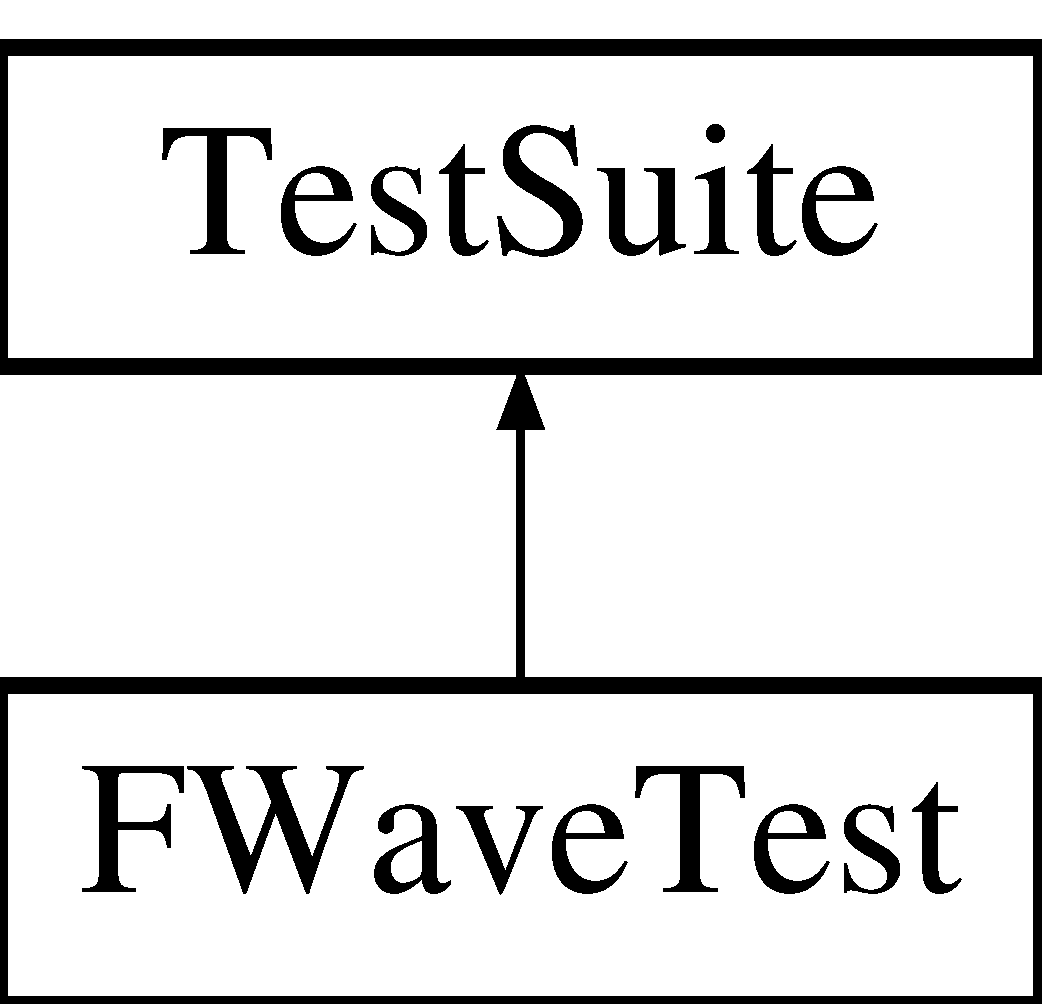
\includegraphics[height=2.000000cm]{classFWaveTest}
\end{center}
\end{figure}
\subsection*{Public Member Functions}
\begin{DoxyCompactItemize}
\item 
\hyperlink{classFWaveTest_a637e3a21850ed7432394b19d1f8320d1}{F\+Wave\+Test} ()
\item 
void \hyperlink{classFWaveTest_aad1779e385672a5fcea0fb09cbd8a2f0}{test\+Same\+Height\+No\+Speed} (void)
\item 
void \hyperlink{classFWaveTest_aed2db9d70b98e7b7924fcb8705bbf509}{test\+Same\+Height\+Left\+Speed} (void)
\item 
void \hyperlink{classFWaveTest_a4cffba9a84aeb963b6b8d4ac79efe227}{test\+Same\+Height\+Right\+Speed} (void)
\item 
void \hyperlink{classFWaveTest_a284fbedaff0f4e2a98ec868926176773}{test\+Same\+Height\+Left\+Right\+Speed} (void)
\item 
void \hyperlink{classFWaveTest_a5ceb6cf106458f0a0110ac13fe2c3f35}{test\+Same\+Height\+Right\+Left\+Speed} (void)
\item 
void \hyperlink{classFWaveTest_abf28f88dc07c66d8ccd7541a2fc9b901}{test\+Decreasing\+Height\+No\+Speed} (void)
\item 
void \hyperlink{classFWaveTest_a817892593d58cf1dad61a2abb0810378}{test\+Decreasing\+Height\+Left\+Speed} (void)
\item 
void \hyperlink{classFWaveTest_aaae1f57e2ef62d53bff1169d84aa7059}{test\+Decreasing\+Height\+Right\+Speed} (void)
\item 
void \hyperlink{classFWaveTest_a2dc496f15de60f5d199d6b1a35b596f3}{test\+Decreasing\+Height\+Left\+Right\+Speed} (void)
\item 
void \hyperlink{classFWaveTest_a24b35d3400c5ee91be94bf7ba47e82bf}{test\+Decreasing\+Height\+Right\+Left\+Speed} (void)
\item 
void \hyperlink{classFWaveTest_abd75e73da77f86f5145dd9ed1796f0fc}{test\+Increasing\+Height\+No\+Speed} (void)
\item 
void \hyperlink{classFWaveTest_aa6a036225ee4f6a00d40ba439899933d}{test\+Increasing\+Height\+Left\+Speed} (void)
\item 
void \hyperlink{classFWaveTest_a3e4e03f910ee006e0dce95cb2276a76a}{test\+Increasing\+Height\+Right\+Speed} (void)
\item 
void \hyperlink{classFWaveTest_a57b9d687f5a7311739883c9931d1e301}{test\+Increasing\+Height\+Left\+Right\+Speed} (void)
\item 
void \hyperlink{classFWaveTest_aaf371e755b499555a6daf142c9e5173f}{test\+Increasing\+Height\+Right\+Left\+Speed} (void)
\item 
void \hyperlink{classFWaveTest_a057ce2e1296eff8b0c0ac4375e138011}{test\+Same\+Bathymethry\+Same\+Height\+Speed\+Right\+Left} (void)
\item 
void \hyperlink{classFWaveTest_ab0572f33ee9ccb4afe2c7baa60d16c0d}{test\+Increasing\+Bathymethry\+Same\+Height\+Speed\+Right} (void)
\item 
void \hyperlink{classFWaveTest_a1c3618e75d53d97441ef3428e772379b}{test\+Increasing\+Bathymethry\+Same\+Height\+Speed\+Left\+Right} (void)
\item 
void \hyperlink{classFWaveTest_a0cf1f7a1f610b71bf50af3f0a63cdbe0}{test\+Increasing\+Bathymethry\+Same\+Height\+Speed\+Right\+Left} (void)
\item 
void \hyperlink{classFWaveTest_a0867052447bec4907c2eca7b88560332}{test\+Decreasing\+Bathymethry\+Same\+Height\+Speed\+Right} (void)
\item 
void \hyperlink{classFWaveTest_ad3749665fb9da5f1a3a8ef91ad18fce6}{test\+Decreasing\+Bathymethry\+Same\+Height\+Speed\+Left\+Right} (void)
\item 
void \hyperlink{classFWaveTest_a3fa1cc4adf7e7b7807639e46e63d17cc}{test\+Decreasing\+Bathymethry\+Same\+Height\+Speed\+Right\+Left} (void)
\item 
void \hyperlink{classFWaveTest_ad1036122e27c158bc42008f4804b9fd2}{test\+Decreasing\+Bathymethry\+Decreasing\+Height\+Speed\+Right\+Stay} (void)
\item 
void \hyperlink{classFWaveTest_abb0e42e169ed6cbc63c9bf76da0da5d4}{test\+Decreasing\+Bathymethry\+Decreasing\+Height\+Speed\+Stay\+Left} (void)
\item 
void \hyperlink{classFWaveTest_a0d88b8b7e5961938c2919d58998d92f5}{test\+Increasing\+Bathymethry\+Decreasing\+Height\+Speed\+Right\+Stay} (void)
\item 
void \hyperlink{classFWaveTest_a0532fd78c0b907b09dc229ca8be2ac81}{test\+Increasing\+Bathymethry\+Decreasing\+Height\+Speed\+Stay\+Left} (void)
\end{DoxyCompactItemize}
\subsection*{Public Attributes}
\begin{DoxyCompactItemize}
\item 
\hyperlink{classsolver_1_1FWave}{solver\+::\+F\+Wave}$<$ T $>$ \hyperlink{classFWaveTest_a195e044738f434127bedf96c2153f230}{fwave}
\end{DoxyCompactItemize}
\subsection*{Static Public Attributes}
\begin{DoxyCompactItemize}
\item 
static const T \hyperlink{classFWaveTest_a8a0b6ebec0c270760dde9af243fc9045}{delta} = 0.\+0001f
\end{DoxyCompactItemize}
\subsection*{Private Attributes}
\begin{DoxyCompactItemize}
\item 
T \hyperlink{classFWaveTest_af8ee955bb870476ec60bd3eabd93434f}{zero}
\end{DoxyCompactItemize}


\subsection{Constructor \& Destructor Documentation}
\hypertarget{classFWaveTest_a637e3a21850ed7432394b19d1f8320d1}{}\index{F\+Wave\+Test@{F\+Wave\+Test}!F\+Wave\+Test@{F\+Wave\+Test}}
\index{F\+Wave\+Test@{F\+Wave\+Test}!F\+Wave\+Test@{F\+Wave\+Test}}
\subsubsection[{F\+Wave\+Test}]{\setlength{\rightskip}{0pt plus 5cm}F\+Wave\+Test\+::\+F\+Wave\+Test (
\begin{DoxyParamCaption}
{}
\end{DoxyParamCaption}
)\hspace{0.3cm}{\ttfamily [inline]}}\label{classFWaveTest_a637e3a21850ed7432394b19d1f8320d1}


\subsection{Member Function Documentation}
\hypertarget{classFWaveTest_ad1036122e27c158bc42008f4804b9fd2}{}\index{F\+Wave\+Test@{F\+Wave\+Test}!test\+Decreasing\+Bathymethry\+Decreasing\+Height\+Speed\+Right\+Stay@{test\+Decreasing\+Bathymethry\+Decreasing\+Height\+Speed\+Right\+Stay}}
\index{test\+Decreasing\+Bathymethry\+Decreasing\+Height\+Speed\+Right\+Stay@{test\+Decreasing\+Bathymethry\+Decreasing\+Height\+Speed\+Right\+Stay}!F\+Wave\+Test@{F\+Wave\+Test}}
\subsubsection[{test\+Decreasing\+Bathymethry\+Decreasing\+Height\+Speed\+Right\+Stay}]{\setlength{\rightskip}{0pt plus 5cm}void F\+Wave\+Test\+::test\+Decreasing\+Bathymethry\+Decreasing\+Height\+Speed\+Right\+Stay (
\begin{DoxyParamCaption}
\item[{void}]{}
\end{DoxyParamCaption}
)\hspace{0.3cm}{\ttfamily [inline]}}\label{classFWaveTest_ad1036122e27c158bc42008f4804b9fd2}
Tests F\+Wave\+::compute\+Net\+Updates with the following parameters\+:~\newline
 hl = 20.\+0~\newline
 hr = 20.\+0~\newline
 ~\newline
 hul = 2.\+0~\newline
 hur = 0.\+0~\newline
 ~\newline
 bl = -\/4.\+0~\newline
 br = -\/2.\+0~\newline
 \hypertarget{classFWaveTest_abb0e42e169ed6cbc63c9bf76da0da5d4}{}\index{F\+Wave\+Test@{F\+Wave\+Test}!test\+Decreasing\+Bathymethry\+Decreasing\+Height\+Speed\+Stay\+Left@{test\+Decreasing\+Bathymethry\+Decreasing\+Height\+Speed\+Stay\+Left}}
\index{test\+Decreasing\+Bathymethry\+Decreasing\+Height\+Speed\+Stay\+Left@{test\+Decreasing\+Bathymethry\+Decreasing\+Height\+Speed\+Stay\+Left}!F\+Wave\+Test@{F\+Wave\+Test}}
\subsubsection[{test\+Decreasing\+Bathymethry\+Decreasing\+Height\+Speed\+Stay\+Left}]{\setlength{\rightskip}{0pt plus 5cm}void F\+Wave\+Test\+::test\+Decreasing\+Bathymethry\+Decreasing\+Height\+Speed\+Stay\+Left (
\begin{DoxyParamCaption}
\item[{void}]{}
\end{DoxyParamCaption}
)\hspace{0.3cm}{\ttfamily [inline]}}\label{classFWaveTest_abb0e42e169ed6cbc63c9bf76da0da5d4}
Tests F\+Wave\+::compute\+Net\+Updates with the following parameters\+:~\newline
 hl = 20.\+0~\newline
 hr = 20.\+0~\newline
 ~\newline
 hul = 0.\+0~\newline
 hur = -\/2.\+0~\newline
 ~\newline
 bl = -\/4.\+0~\newline
 br = -\/2.\+0~\newline
 \hypertarget{classFWaveTest_ad3749665fb9da5f1a3a8ef91ad18fce6}{}\index{F\+Wave\+Test@{F\+Wave\+Test}!test\+Decreasing\+Bathymethry\+Same\+Height\+Speed\+Left\+Right@{test\+Decreasing\+Bathymethry\+Same\+Height\+Speed\+Left\+Right}}
\index{test\+Decreasing\+Bathymethry\+Same\+Height\+Speed\+Left\+Right@{test\+Decreasing\+Bathymethry\+Same\+Height\+Speed\+Left\+Right}!F\+Wave\+Test@{F\+Wave\+Test}}
\subsubsection[{test\+Decreasing\+Bathymethry\+Same\+Height\+Speed\+Left\+Right}]{\setlength{\rightskip}{0pt plus 5cm}void F\+Wave\+Test\+::test\+Decreasing\+Bathymethry\+Same\+Height\+Speed\+Left\+Right (
\begin{DoxyParamCaption}
\item[{void}]{}
\end{DoxyParamCaption}
)\hspace{0.3cm}{\ttfamily [inline]}}\label{classFWaveTest_ad3749665fb9da5f1a3a8ef91ad18fce6}
Tests F\+Wave\+::compute\+Net\+Updates with the following parameters\+:~\newline
 hl = 4.\+0~\newline
 hr = 6.\+0~\newline
 ~\newline
 hul = -\/2.\+0~\newline
 hur = 2.\+0~\newline
 ~\newline
 bl = -\/4.\+0~\newline
 br = -\/2.\+0~\newline
 \hypertarget{classFWaveTest_a0867052447bec4907c2eca7b88560332}{}\index{F\+Wave\+Test@{F\+Wave\+Test}!test\+Decreasing\+Bathymethry\+Same\+Height\+Speed\+Right@{test\+Decreasing\+Bathymethry\+Same\+Height\+Speed\+Right}}
\index{test\+Decreasing\+Bathymethry\+Same\+Height\+Speed\+Right@{test\+Decreasing\+Bathymethry\+Same\+Height\+Speed\+Right}!F\+Wave\+Test@{F\+Wave\+Test}}
\subsubsection[{test\+Decreasing\+Bathymethry\+Same\+Height\+Speed\+Right}]{\setlength{\rightskip}{0pt plus 5cm}void F\+Wave\+Test\+::test\+Decreasing\+Bathymethry\+Same\+Height\+Speed\+Right (
\begin{DoxyParamCaption}
\item[{void}]{}
\end{DoxyParamCaption}
)\hspace{0.3cm}{\ttfamily [inline]}}\label{classFWaveTest_a0867052447bec4907c2eca7b88560332}
Tests F\+Wave\+::compute\+Net\+Updates with the following parameters\+:~\newline
 hl = 4.\+0~\newline
 hr = 6.\+0~\newline
 ~\newline
 hul = 2.\+0~\newline
 hur = 2.\+0~\newline
 ~\newline
 bl = -\/4.\+0~\newline
 br = -\/2.\+0~\newline
 \hypertarget{classFWaveTest_a3fa1cc4adf7e7b7807639e46e63d17cc}{}\index{F\+Wave\+Test@{F\+Wave\+Test}!test\+Decreasing\+Bathymethry\+Same\+Height\+Speed\+Right\+Left@{test\+Decreasing\+Bathymethry\+Same\+Height\+Speed\+Right\+Left}}
\index{test\+Decreasing\+Bathymethry\+Same\+Height\+Speed\+Right\+Left@{test\+Decreasing\+Bathymethry\+Same\+Height\+Speed\+Right\+Left}!F\+Wave\+Test@{F\+Wave\+Test}}
\subsubsection[{test\+Decreasing\+Bathymethry\+Same\+Height\+Speed\+Right\+Left}]{\setlength{\rightskip}{0pt plus 5cm}void F\+Wave\+Test\+::test\+Decreasing\+Bathymethry\+Same\+Height\+Speed\+Right\+Left (
\begin{DoxyParamCaption}
\item[{void}]{}
\end{DoxyParamCaption}
)\hspace{0.3cm}{\ttfamily [inline]}}\label{classFWaveTest_a3fa1cc4adf7e7b7807639e46e63d17cc}
Tests F\+Wave\+::compute\+Net\+Updates with the following parameters\+:~\newline
 hl = 4.\+0~\newline
 hr = 6.\+0~\newline
 ~\newline
 hul = 2.\+0~\newline
 hur = -\/2.\+0~\newline
 ~\newline
 bl = -\/4.\+0~\newline
 br = -\/2.\+0~\newline
 \hypertarget{classFWaveTest_a2dc496f15de60f5d199d6b1a35b596f3}{}\index{F\+Wave\+Test@{F\+Wave\+Test}!test\+Decreasing\+Height\+Left\+Right\+Speed@{test\+Decreasing\+Height\+Left\+Right\+Speed}}
\index{test\+Decreasing\+Height\+Left\+Right\+Speed@{test\+Decreasing\+Height\+Left\+Right\+Speed}!F\+Wave\+Test@{F\+Wave\+Test}}
\subsubsection[{test\+Decreasing\+Height\+Left\+Right\+Speed}]{\setlength{\rightskip}{0pt plus 5cm}void F\+Wave\+Test\+::test\+Decreasing\+Height\+Left\+Right\+Speed (
\begin{DoxyParamCaption}
\item[{void}]{}
\end{DoxyParamCaption}
)\hspace{0.3cm}{\ttfamily [inline]}}\label{classFWaveTest_a2dc496f15de60f5d199d6b1a35b596f3}
Tests F\+Wave\+::compute\+Net\+Updates with the following parameters\+:~\newline
 hl = 10.\+0~\newline
 hr = 5.\+0~\newline
 ~\newline
 hul = -\/2.\+0~\newline
 hur = 3.\+0~\newline
 ~\newline
 bl = 0~\newline
 br = 0~\newline
 \hypertarget{classFWaveTest_a817892593d58cf1dad61a2abb0810378}{}\index{F\+Wave\+Test@{F\+Wave\+Test}!test\+Decreasing\+Height\+Left\+Speed@{test\+Decreasing\+Height\+Left\+Speed}}
\index{test\+Decreasing\+Height\+Left\+Speed@{test\+Decreasing\+Height\+Left\+Speed}!F\+Wave\+Test@{F\+Wave\+Test}}
\subsubsection[{test\+Decreasing\+Height\+Left\+Speed}]{\setlength{\rightskip}{0pt plus 5cm}void F\+Wave\+Test\+::test\+Decreasing\+Height\+Left\+Speed (
\begin{DoxyParamCaption}
\item[{void}]{}
\end{DoxyParamCaption}
)\hspace{0.3cm}{\ttfamily [inline]}}\label{classFWaveTest_a817892593d58cf1dad61a2abb0810378}
Tests F\+Wave\+::compute\+Net\+Updates with the following parameters\+:~\newline
 hl = 10.\+0~\newline
 hr = 5.\+0~\newline
 ~\newline
 hul = -\/2.\+0~\newline
 hur = -\/3.\+0~\newline
 ~\newline
 bl = 0~\newline
 br = 0~\newline
 \hypertarget{classFWaveTest_abf28f88dc07c66d8ccd7541a2fc9b901}{}\index{F\+Wave\+Test@{F\+Wave\+Test}!test\+Decreasing\+Height\+No\+Speed@{test\+Decreasing\+Height\+No\+Speed}}
\index{test\+Decreasing\+Height\+No\+Speed@{test\+Decreasing\+Height\+No\+Speed}!F\+Wave\+Test@{F\+Wave\+Test}}
\subsubsection[{test\+Decreasing\+Height\+No\+Speed}]{\setlength{\rightskip}{0pt plus 5cm}void F\+Wave\+Test\+::test\+Decreasing\+Height\+No\+Speed (
\begin{DoxyParamCaption}
\item[{void}]{}
\end{DoxyParamCaption}
)\hspace{0.3cm}{\ttfamily [inline]}}\label{classFWaveTest_abf28f88dc07c66d8ccd7541a2fc9b901}
Tests F\+Wave\+::compute\+Net\+Updates with the following parameters\+:~\newline
 hl = 10.\+0~\newline
 hr = 5.\+0~\newline
 ~\newline
 hul = 0~\newline
 hur = 0~\newline
 ~\newline
 bl = 0~\newline
 br = 0~\newline
 \hypertarget{classFWaveTest_a24b35d3400c5ee91be94bf7ba47e82bf}{}\index{F\+Wave\+Test@{F\+Wave\+Test}!test\+Decreasing\+Height\+Right\+Left\+Speed@{test\+Decreasing\+Height\+Right\+Left\+Speed}}
\index{test\+Decreasing\+Height\+Right\+Left\+Speed@{test\+Decreasing\+Height\+Right\+Left\+Speed}!F\+Wave\+Test@{F\+Wave\+Test}}
\subsubsection[{test\+Decreasing\+Height\+Right\+Left\+Speed}]{\setlength{\rightskip}{0pt plus 5cm}void F\+Wave\+Test\+::test\+Decreasing\+Height\+Right\+Left\+Speed (
\begin{DoxyParamCaption}
\item[{void}]{}
\end{DoxyParamCaption}
)\hspace{0.3cm}{\ttfamily [inline]}}\label{classFWaveTest_a24b35d3400c5ee91be94bf7ba47e82bf}
Tests F\+Wave\+::compute\+Net\+Updates with the following parameters\+:~\newline
 hl = 10.\+0~\newline
 hr = 5.\+0~\newline
 ~\newline
 hul = 3.\+0~\newline
 hur = -\/2.\+0~\newline
 ~\newline
 bl = 0~\newline
 br = 0~\newline
 \hypertarget{classFWaveTest_aaae1f57e2ef62d53bff1169d84aa7059}{}\index{F\+Wave\+Test@{F\+Wave\+Test}!test\+Decreasing\+Height\+Right\+Speed@{test\+Decreasing\+Height\+Right\+Speed}}
\index{test\+Decreasing\+Height\+Right\+Speed@{test\+Decreasing\+Height\+Right\+Speed}!F\+Wave\+Test@{F\+Wave\+Test}}
\subsubsection[{test\+Decreasing\+Height\+Right\+Speed}]{\setlength{\rightskip}{0pt plus 5cm}void F\+Wave\+Test\+::test\+Decreasing\+Height\+Right\+Speed (
\begin{DoxyParamCaption}
\item[{void}]{}
\end{DoxyParamCaption}
)\hspace{0.3cm}{\ttfamily [inline]}}\label{classFWaveTest_aaae1f57e2ef62d53bff1169d84aa7059}
Tests F\+Wave\+::compute\+Net\+Updates with the following parameters\+:~\newline
 hl = 10.\+0~\newline
 hr = 5.\+0~\newline
 ~\newline
 hul = 3.\+0~\newline
 hur = 2.\+0~\newline
 ~\newline
 bl = 0~\newline
 br = 0~\newline
 \hypertarget{classFWaveTest_a0d88b8b7e5961938c2919d58998d92f5}{}\index{F\+Wave\+Test@{F\+Wave\+Test}!test\+Increasing\+Bathymethry\+Decreasing\+Height\+Speed\+Right\+Stay@{test\+Increasing\+Bathymethry\+Decreasing\+Height\+Speed\+Right\+Stay}}
\index{test\+Increasing\+Bathymethry\+Decreasing\+Height\+Speed\+Right\+Stay@{test\+Increasing\+Bathymethry\+Decreasing\+Height\+Speed\+Right\+Stay}!F\+Wave\+Test@{F\+Wave\+Test}}
\subsubsection[{test\+Increasing\+Bathymethry\+Decreasing\+Height\+Speed\+Right\+Stay}]{\setlength{\rightskip}{0pt plus 5cm}void F\+Wave\+Test\+::test\+Increasing\+Bathymethry\+Decreasing\+Height\+Speed\+Right\+Stay (
\begin{DoxyParamCaption}
\item[{void}]{}
\end{DoxyParamCaption}
)\hspace{0.3cm}{\ttfamily [inline]}}\label{classFWaveTest_a0d88b8b7e5961938c2919d58998d92f5}
Tests F\+Wave\+::compute\+Net\+Updates with the following parameters\+:~\newline
 hl = 20.\+0~\newline
 hr = 16.\+0~\newline
 ~\newline
 hul = 2.\+0~\newline
 hur = 0.\+0~\newline
 ~\newline
 bl = -\/2.\+0~\newline
 br = -\/4.\+0~\newline
 \hypertarget{classFWaveTest_a0532fd78c0b907b09dc229ca8be2ac81}{}\index{F\+Wave\+Test@{F\+Wave\+Test}!test\+Increasing\+Bathymethry\+Decreasing\+Height\+Speed\+Stay\+Left@{test\+Increasing\+Bathymethry\+Decreasing\+Height\+Speed\+Stay\+Left}}
\index{test\+Increasing\+Bathymethry\+Decreasing\+Height\+Speed\+Stay\+Left@{test\+Increasing\+Bathymethry\+Decreasing\+Height\+Speed\+Stay\+Left}!F\+Wave\+Test@{F\+Wave\+Test}}
\subsubsection[{test\+Increasing\+Bathymethry\+Decreasing\+Height\+Speed\+Stay\+Left}]{\setlength{\rightskip}{0pt plus 5cm}void F\+Wave\+Test\+::test\+Increasing\+Bathymethry\+Decreasing\+Height\+Speed\+Stay\+Left (
\begin{DoxyParamCaption}
\item[{void}]{}
\end{DoxyParamCaption}
)\hspace{0.3cm}{\ttfamily [inline]}}\label{classFWaveTest_a0532fd78c0b907b09dc229ca8be2ac81}
Tests F\+Wave\+::compute\+Net\+Updates with the following parameters\+:~\newline
 hl = 20.\+0~\newline
 hr = 16.\+0~\newline
 ~\newline
 hul = 0.\+0~\newline
 hur = -\/2.\+0~\newline
 ~\newline
 bl = -\/2.\+0~\newline
 br = -\/4.\+0~\newline
 \hypertarget{classFWaveTest_a1c3618e75d53d97441ef3428e772379b}{}\index{F\+Wave\+Test@{F\+Wave\+Test}!test\+Increasing\+Bathymethry\+Same\+Height\+Speed\+Left\+Right@{test\+Increasing\+Bathymethry\+Same\+Height\+Speed\+Left\+Right}}
\index{test\+Increasing\+Bathymethry\+Same\+Height\+Speed\+Left\+Right@{test\+Increasing\+Bathymethry\+Same\+Height\+Speed\+Left\+Right}!F\+Wave\+Test@{F\+Wave\+Test}}
\subsubsection[{test\+Increasing\+Bathymethry\+Same\+Height\+Speed\+Left\+Right}]{\setlength{\rightskip}{0pt plus 5cm}void F\+Wave\+Test\+::test\+Increasing\+Bathymethry\+Same\+Height\+Speed\+Left\+Right (
\begin{DoxyParamCaption}
\item[{void}]{}
\end{DoxyParamCaption}
)\hspace{0.3cm}{\ttfamily [inline]}}\label{classFWaveTest_a1c3618e75d53d97441ef3428e772379b}
Tests F\+Wave\+::compute\+Net\+Updates with the following parameters\+:~\newline
 hl = 6.\+0~\newline
 hr = 4.\+0~\newline
 ~\newline
 hul = -\/2.\+0~\newline
 hur = 2.\+0~\newline
 ~\newline
 bl = -\/2.\+0~\newline
 br = -\/4.\+0~\newline
 \hypertarget{classFWaveTest_ab0572f33ee9ccb4afe2c7baa60d16c0d}{}\index{F\+Wave\+Test@{F\+Wave\+Test}!test\+Increasing\+Bathymethry\+Same\+Height\+Speed\+Right@{test\+Increasing\+Bathymethry\+Same\+Height\+Speed\+Right}}
\index{test\+Increasing\+Bathymethry\+Same\+Height\+Speed\+Right@{test\+Increasing\+Bathymethry\+Same\+Height\+Speed\+Right}!F\+Wave\+Test@{F\+Wave\+Test}}
\subsubsection[{test\+Increasing\+Bathymethry\+Same\+Height\+Speed\+Right}]{\setlength{\rightskip}{0pt plus 5cm}void F\+Wave\+Test\+::test\+Increasing\+Bathymethry\+Same\+Height\+Speed\+Right (
\begin{DoxyParamCaption}
\item[{void}]{}
\end{DoxyParamCaption}
)\hspace{0.3cm}{\ttfamily [inline]}}\label{classFWaveTest_ab0572f33ee9ccb4afe2c7baa60d16c0d}
Tests F\+Wave\+::compute\+Net\+Updates with the following parameters\+:~\newline
 hl = 6.\+0~\newline
 hr = 4.\+0~\newline
 ~\newline
 hul = 2.\+0~\newline
 hur = 2.\+0~\newline
 ~\newline
 bl = -\/2.\+0~\newline
 br = -\/4.\+0~\newline
 \hypertarget{classFWaveTest_a0cf1f7a1f610b71bf50af3f0a63cdbe0}{}\index{F\+Wave\+Test@{F\+Wave\+Test}!test\+Increasing\+Bathymethry\+Same\+Height\+Speed\+Right\+Left@{test\+Increasing\+Bathymethry\+Same\+Height\+Speed\+Right\+Left}}
\index{test\+Increasing\+Bathymethry\+Same\+Height\+Speed\+Right\+Left@{test\+Increasing\+Bathymethry\+Same\+Height\+Speed\+Right\+Left}!F\+Wave\+Test@{F\+Wave\+Test}}
\subsubsection[{test\+Increasing\+Bathymethry\+Same\+Height\+Speed\+Right\+Left}]{\setlength{\rightskip}{0pt plus 5cm}void F\+Wave\+Test\+::test\+Increasing\+Bathymethry\+Same\+Height\+Speed\+Right\+Left (
\begin{DoxyParamCaption}
\item[{void}]{}
\end{DoxyParamCaption}
)\hspace{0.3cm}{\ttfamily [inline]}}\label{classFWaveTest_a0cf1f7a1f610b71bf50af3f0a63cdbe0}
Tests F\+Wave\+::compute\+Net\+Updates with the following parameters\+:~\newline
 hl = 6.\+0~\newline
 hr = 4.\+0~\newline
 ~\newline
 hul = 2.\+0~\newline
 hur = -\/2.\+0~\newline
 ~\newline
 bl = -\/2.\+0~\newline
 br = -\/4.\+0~\newline
 \hypertarget{classFWaveTest_a57b9d687f5a7311739883c9931d1e301}{}\index{F\+Wave\+Test@{F\+Wave\+Test}!test\+Increasing\+Height\+Left\+Right\+Speed@{test\+Increasing\+Height\+Left\+Right\+Speed}}
\index{test\+Increasing\+Height\+Left\+Right\+Speed@{test\+Increasing\+Height\+Left\+Right\+Speed}!F\+Wave\+Test@{F\+Wave\+Test}}
\subsubsection[{test\+Increasing\+Height\+Left\+Right\+Speed}]{\setlength{\rightskip}{0pt plus 5cm}void F\+Wave\+Test\+::test\+Increasing\+Height\+Left\+Right\+Speed (
\begin{DoxyParamCaption}
\item[{void}]{}
\end{DoxyParamCaption}
)\hspace{0.3cm}{\ttfamily [inline]}}\label{classFWaveTest_a57b9d687f5a7311739883c9931d1e301}
Tests F\+Wave\+::compute\+Net\+Updates with the following parameters\+:~\newline
 hl = 5.\+0~\newline
 hr = 10.\+0~\newline
 ~\newline
 hul = -\/3.\+0~\newline
 hur = 2.\+0~\newline
 ~\newline
 bl = 0~\newline
 br = 0~\newline
 \hypertarget{classFWaveTest_aa6a036225ee4f6a00d40ba439899933d}{}\index{F\+Wave\+Test@{F\+Wave\+Test}!test\+Increasing\+Height\+Left\+Speed@{test\+Increasing\+Height\+Left\+Speed}}
\index{test\+Increasing\+Height\+Left\+Speed@{test\+Increasing\+Height\+Left\+Speed}!F\+Wave\+Test@{F\+Wave\+Test}}
\subsubsection[{test\+Increasing\+Height\+Left\+Speed}]{\setlength{\rightskip}{0pt plus 5cm}void F\+Wave\+Test\+::test\+Increasing\+Height\+Left\+Speed (
\begin{DoxyParamCaption}
\item[{void}]{}
\end{DoxyParamCaption}
)\hspace{0.3cm}{\ttfamily [inline]}}\label{classFWaveTest_aa6a036225ee4f6a00d40ba439899933d}
Tests F\+Wave\+::compute\+Net\+Updates with the following parameters\+:~\newline
 hl = 5.\+0~\newline
 hr = 10.\+0~\newline
 ~\newline
 hul = -\/3.\+0~\newline
 hur = -\/2.\+0~\newline
 ~\newline
 bl = 0~\newline
 br = 0~\newline
 \hypertarget{classFWaveTest_abd75e73da77f86f5145dd9ed1796f0fc}{}\index{F\+Wave\+Test@{F\+Wave\+Test}!test\+Increasing\+Height\+No\+Speed@{test\+Increasing\+Height\+No\+Speed}}
\index{test\+Increasing\+Height\+No\+Speed@{test\+Increasing\+Height\+No\+Speed}!F\+Wave\+Test@{F\+Wave\+Test}}
\subsubsection[{test\+Increasing\+Height\+No\+Speed}]{\setlength{\rightskip}{0pt plus 5cm}void F\+Wave\+Test\+::test\+Increasing\+Height\+No\+Speed (
\begin{DoxyParamCaption}
\item[{void}]{}
\end{DoxyParamCaption}
)\hspace{0.3cm}{\ttfamily [inline]}}\label{classFWaveTest_abd75e73da77f86f5145dd9ed1796f0fc}
Tests F\+Wave\+::compute\+Net\+Updates with the following parameters\+:~\newline
 hl = 5.\+0~\newline
 hr = 10.\+0~\newline
 ~\newline
 hul = 0~\newline
 hur = 0~\newline
 ~\newline
 bl = 0~\newline
 br = 0~\newline
 \hypertarget{classFWaveTest_aaf371e755b499555a6daf142c9e5173f}{}\index{F\+Wave\+Test@{F\+Wave\+Test}!test\+Increasing\+Height\+Right\+Left\+Speed@{test\+Increasing\+Height\+Right\+Left\+Speed}}
\index{test\+Increasing\+Height\+Right\+Left\+Speed@{test\+Increasing\+Height\+Right\+Left\+Speed}!F\+Wave\+Test@{F\+Wave\+Test}}
\subsubsection[{test\+Increasing\+Height\+Right\+Left\+Speed}]{\setlength{\rightskip}{0pt plus 5cm}void F\+Wave\+Test\+::test\+Increasing\+Height\+Right\+Left\+Speed (
\begin{DoxyParamCaption}
\item[{void}]{}
\end{DoxyParamCaption}
)\hspace{0.3cm}{\ttfamily [inline]}}\label{classFWaveTest_aaf371e755b499555a6daf142c9e5173f}
Tests F\+Wave\+::compute\+Net\+Updates with the following parameters\+:~\newline
 hl = 5.\+0~\newline
 hr = 10.\+0~\newline
 ~\newline
 hul = 2.\+0~\newline
 hur = -\/3.\+0~\newline
 ~\newline
 bl = 0~\newline
 br = 0~\newline
 \hypertarget{classFWaveTest_a3e4e03f910ee006e0dce95cb2276a76a}{}\index{F\+Wave\+Test@{F\+Wave\+Test}!test\+Increasing\+Height\+Right\+Speed@{test\+Increasing\+Height\+Right\+Speed}}
\index{test\+Increasing\+Height\+Right\+Speed@{test\+Increasing\+Height\+Right\+Speed}!F\+Wave\+Test@{F\+Wave\+Test}}
\subsubsection[{test\+Increasing\+Height\+Right\+Speed}]{\setlength{\rightskip}{0pt plus 5cm}void F\+Wave\+Test\+::test\+Increasing\+Height\+Right\+Speed (
\begin{DoxyParamCaption}
\item[{void}]{}
\end{DoxyParamCaption}
)\hspace{0.3cm}{\ttfamily [inline]}}\label{classFWaveTest_a3e4e03f910ee006e0dce95cb2276a76a}
Tests F\+Wave\+::compute\+Net\+Updates with the following parameters\+:~\newline
 hl = 5.\+0~\newline
 hr = 10.\+0~\newline
 ~\newline
 hul = 2.\+0~\newline
 hur = 3.\+0~\newline
 ~\newline
 bl = 0~\newline
 br = 0~\newline
 \hypertarget{classFWaveTest_a057ce2e1296eff8b0c0ac4375e138011}{}\index{F\+Wave\+Test@{F\+Wave\+Test}!test\+Same\+Bathymethry\+Same\+Height\+Speed\+Right\+Left@{test\+Same\+Bathymethry\+Same\+Height\+Speed\+Right\+Left}}
\index{test\+Same\+Bathymethry\+Same\+Height\+Speed\+Right\+Left@{test\+Same\+Bathymethry\+Same\+Height\+Speed\+Right\+Left}!F\+Wave\+Test@{F\+Wave\+Test}}
\subsubsection[{test\+Same\+Bathymethry\+Same\+Height\+Speed\+Right\+Left}]{\setlength{\rightskip}{0pt plus 5cm}void F\+Wave\+Test\+::test\+Same\+Bathymethry\+Same\+Height\+Speed\+Right\+Left (
\begin{DoxyParamCaption}
\item[{void}]{}
\end{DoxyParamCaption}
)\hspace{0.3cm}{\ttfamily [inline]}}\label{classFWaveTest_a057ce2e1296eff8b0c0ac4375e138011}
Tests F\+Wave\+::compute\+Net\+Updates with the following parameters\+:~\newline
 hl = 6.\+0~\newline
 hr = 6.\+0~\newline
 ~\newline
 hul = 2.\+0~\newline
 hur = 2.\+0~\newline
 ~\newline
 bl = -\/4.\+0~\newline
 br = -\/4.\+0~\newline
 \hypertarget{classFWaveTest_a284fbedaff0f4e2a98ec868926176773}{}\index{F\+Wave\+Test@{F\+Wave\+Test}!test\+Same\+Height\+Left\+Right\+Speed@{test\+Same\+Height\+Left\+Right\+Speed}}
\index{test\+Same\+Height\+Left\+Right\+Speed@{test\+Same\+Height\+Left\+Right\+Speed}!F\+Wave\+Test@{F\+Wave\+Test}}
\subsubsection[{test\+Same\+Height\+Left\+Right\+Speed}]{\setlength{\rightskip}{0pt plus 5cm}void F\+Wave\+Test\+::test\+Same\+Height\+Left\+Right\+Speed (
\begin{DoxyParamCaption}
\item[{void}]{}
\end{DoxyParamCaption}
)\hspace{0.3cm}{\ttfamily [inline]}}\label{classFWaveTest_a284fbedaff0f4e2a98ec868926176773}
Tests F\+Wave\+::compute\+Net\+Updates with the following parameters\+:~\newline
 hl = 5.\+0~\newline
 hr = 5.\+0~\newline
 ~\newline
 hul = -\/3.\+0~\newline
 hur = 2.\+0~\newline
 ~\newline
 bl = 0~\newline
 br = 0~\newline
 \hypertarget{classFWaveTest_aed2db9d70b98e7b7924fcb8705bbf509}{}\index{F\+Wave\+Test@{F\+Wave\+Test}!test\+Same\+Height\+Left\+Speed@{test\+Same\+Height\+Left\+Speed}}
\index{test\+Same\+Height\+Left\+Speed@{test\+Same\+Height\+Left\+Speed}!F\+Wave\+Test@{F\+Wave\+Test}}
\subsubsection[{test\+Same\+Height\+Left\+Speed}]{\setlength{\rightskip}{0pt plus 5cm}void F\+Wave\+Test\+::test\+Same\+Height\+Left\+Speed (
\begin{DoxyParamCaption}
\item[{void}]{}
\end{DoxyParamCaption}
)\hspace{0.3cm}{\ttfamily [inline]}}\label{classFWaveTest_aed2db9d70b98e7b7924fcb8705bbf509}
Tests F\+Wave\+::compute\+Net\+Updates with the following parameters\+:~\newline
 hl = 5.\+0~\newline
 hr = 5.\+0~\newline
 ~\newline
 hul = -\/2.\+0~\newline
 hur = -\/3.\+0~\newline
 ~\newline
 bl = 0~\newline
 br = 0~\newline
 \hypertarget{classFWaveTest_aad1779e385672a5fcea0fb09cbd8a2f0}{}\index{F\+Wave\+Test@{F\+Wave\+Test}!test\+Same\+Height\+No\+Speed@{test\+Same\+Height\+No\+Speed}}
\index{test\+Same\+Height\+No\+Speed@{test\+Same\+Height\+No\+Speed}!F\+Wave\+Test@{F\+Wave\+Test}}
\subsubsection[{test\+Same\+Height\+No\+Speed}]{\setlength{\rightskip}{0pt plus 5cm}void F\+Wave\+Test\+::test\+Same\+Height\+No\+Speed (
\begin{DoxyParamCaption}
\item[{void}]{}
\end{DoxyParamCaption}
)\hspace{0.3cm}{\ttfamily [inline]}}\label{classFWaveTest_aad1779e385672a5fcea0fb09cbd8a2f0}
Tests F\+Wave\+::compute\+Net\+Updates with the following parameters\+:~\newline
 hl = 5.\+0~\newline
 hr = 5.\+0~\newline
 ~\newline
 hul = 0~\newline
 hur = 0~\newline
 ~\newline
 bl = 0~\newline
 br = 0~\newline
 \hypertarget{classFWaveTest_a5ceb6cf106458f0a0110ac13fe2c3f35}{}\index{F\+Wave\+Test@{F\+Wave\+Test}!test\+Same\+Height\+Right\+Left\+Speed@{test\+Same\+Height\+Right\+Left\+Speed}}
\index{test\+Same\+Height\+Right\+Left\+Speed@{test\+Same\+Height\+Right\+Left\+Speed}!F\+Wave\+Test@{F\+Wave\+Test}}
\subsubsection[{test\+Same\+Height\+Right\+Left\+Speed}]{\setlength{\rightskip}{0pt plus 5cm}void F\+Wave\+Test\+::test\+Same\+Height\+Right\+Left\+Speed (
\begin{DoxyParamCaption}
\item[{void}]{}
\end{DoxyParamCaption}
)\hspace{0.3cm}{\ttfamily [inline]}}\label{classFWaveTest_a5ceb6cf106458f0a0110ac13fe2c3f35}
Tests F\+Wave\+::compute\+Net\+Updates with the following parameters\+:~\newline
 hl = 5.\+0~\newline
 hr = 5.\+0~\newline
 ~\newline
 hul = 2.\+0~\newline
 hur = -\/3.\+0~\newline
 ~\newline
 bl = 0~\newline
 br = 0~\newline
 \hypertarget{classFWaveTest_a4cffba9a84aeb963b6b8d4ac79efe227}{}\index{F\+Wave\+Test@{F\+Wave\+Test}!test\+Same\+Height\+Right\+Speed@{test\+Same\+Height\+Right\+Speed}}
\index{test\+Same\+Height\+Right\+Speed@{test\+Same\+Height\+Right\+Speed}!F\+Wave\+Test@{F\+Wave\+Test}}
\subsubsection[{test\+Same\+Height\+Right\+Speed}]{\setlength{\rightskip}{0pt plus 5cm}void F\+Wave\+Test\+::test\+Same\+Height\+Right\+Speed (
\begin{DoxyParamCaption}
\item[{void}]{}
\end{DoxyParamCaption}
)\hspace{0.3cm}{\ttfamily [inline]}}\label{classFWaveTest_a4cffba9a84aeb963b6b8d4ac79efe227}
Tests F\+Wave\+::compute\+Net\+Updates with the following parameters\+:~\newline
 hl = 5.\+0~\newline
 hr = 5.\+0~\newline
 ~\newline
 hul = 3.\+0~\newline
 hur = 2.\+0~\newline
 ~\newline
 bl = 0~\newline
 br = 0~\newline
 

\subsection{Member Data Documentation}
\hypertarget{classFWaveTest_a8a0b6ebec0c270760dde9af243fc9045}{}\index{F\+Wave\+Test@{F\+Wave\+Test}!delta@{delta}}
\index{delta@{delta}!F\+Wave\+Test@{F\+Wave\+Test}}
\subsubsection[{delta}]{\setlength{\rightskip}{0pt plus 5cm}const T F\+Wave\+Test\+::delta = 0.\+0001f\hspace{0.3cm}{\ttfamily [static]}}\label{classFWaveTest_a8a0b6ebec0c270760dde9af243fc9045}
Delta used for comparing expected and actual values \hypertarget{classFWaveTest_a195e044738f434127bedf96c2153f230}{}\index{F\+Wave\+Test@{F\+Wave\+Test}!fwave@{fwave}}
\index{fwave@{fwave}!F\+Wave\+Test@{F\+Wave\+Test}}
\subsubsection[{fwave}]{\setlength{\rightskip}{0pt plus 5cm}{\bf solver\+::\+F\+Wave}$<$T$>$ F\+Wave\+Test\+::fwave}\label{classFWaveTest_a195e044738f434127bedf96c2153f230}
F\+Wave to test \hypertarget{classFWaveTest_af8ee955bb870476ec60bd3eabd93434f}{}\index{F\+Wave\+Test@{F\+Wave\+Test}!zero@{zero}}
\index{zero@{zero}!F\+Wave\+Test@{F\+Wave\+Test}}
\subsubsection[{zero}]{\setlength{\rightskip}{0pt plus 5cm}T F\+Wave\+Test\+::zero\hspace{0.3cm}{\ttfamily [private]}}\label{classFWaveTest_af8ee955bb870476ec60bd3eabd93434f}
Zero\+: 0.\+0f 

The documentation for this class was generated from the following file\+:\begin{DoxyCompactItemize}
\item 
\hyperlink{FWaveTest_8h}{F\+Wave\+Test.\+h}\end{DoxyCompactItemize}

\hypertarget{structsolver_1_1FWave_1_1Quantity}{}\section{solver\+:\+:F\+Wave$<$ T $>$\+:\+:Quantity Struct Reference}
\label{structsolver_1_1FWave_1_1Quantity}\index{solver\+::\+F\+Wave$<$ T $>$\+::\+Quantity@{solver\+::\+F\+Wave$<$ T $>$\+::\+Quantity}}


{\ttfamily \#include $<$F\+Wave.\+hpp$>$}

\subsection*{Public Attributes}
\begin{DoxyCompactItemize}
\item 
T \hyperlink{structsolver_1_1FWave_1_1Quantity_ab21e966b42ed55a04b852deb96ec7285}{h}
\item 
T \hyperlink{structsolver_1_1FWave_1_1Quantity_a85b3d7be51ca5dc26a031d421c16095c}{hu}
\end{DoxyCompactItemize}


\subsection{Member Data Documentation}
\hypertarget{structsolver_1_1FWave_1_1Quantity_ab21e966b42ed55a04b852deb96ec7285}{}\index{solver\+::\+F\+Wave\+::\+Quantity@{solver\+::\+F\+Wave\+::\+Quantity}!h@{h}}
\index{h@{h}!solver\+::\+F\+Wave\+::\+Quantity@{solver\+::\+F\+Wave\+::\+Quantity}}
\subsubsection[{h}]{\setlength{\rightskip}{0pt plus 5cm}template$<$typename T$>$ T {\bf solver\+::\+F\+Wave}$<$ T $>$\+::Quantity\+::h}\label{structsolver_1_1FWave_1_1Quantity_ab21e966b42ed55a04b852deb96ec7285}
\hypertarget{structsolver_1_1FWave_1_1Quantity_a85b3d7be51ca5dc26a031d421c16095c}{}\index{solver\+::\+F\+Wave\+::\+Quantity@{solver\+::\+F\+Wave\+::\+Quantity}!hu@{hu}}
\index{hu@{hu}!solver\+::\+F\+Wave\+::\+Quantity@{solver\+::\+F\+Wave\+::\+Quantity}}
\subsubsection[{hu}]{\setlength{\rightskip}{0pt plus 5cm}template$<$typename T$>$ T {\bf solver\+::\+F\+Wave}$<$ T $>$\+::Quantity\+::hu}\label{structsolver_1_1FWave_1_1Quantity_a85b3d7be51ca5dc26a031d421c16095c}


The documentation for this struct was generated from the following file\+:\begin{DoxyCompactItemize}
\item 
\hyperlink{FWave_8hpp}{F\+Wave.\+hpp}\end{DoxyCompactItemize}

\chapter{File Documentation}
\hypertarget{FWave_8hpp}{}\section{F\+Wave.\+hpp File Reference}
\label{FWave_8hpp}\index{F\+Wave.\+hpp@{F\+Wave.\+hpp}}
{\ttfamily \#include $<$cassert$>$}\\*
{\ttfamily \#include $<$cmath$>$}\\*
{\ttfamily \#include $<$iostream$>$}\\*
\subsection*{Classes}
\begin{DoxyCompactItemize}
\item 
class \hyperlink{classsolver_1_1FWave}{solver\+::\+F\+Wave$<$ T $>$}
\item 
class \hyperlink{classsolver_1_1FWave}{solver\+::\+F\+Wave$<$ T $>$}
\item 
struct \hyperlink{structsolver_1_1FWave_1_1Quantity}{solver\+::\+F\+Wave$<$ T $>$\+::\+Quantity}
\end{DoxyCompactItemize}
\subsection*{Namespaces}
\begin{DoxyCompactItemize}
\item 
 \hyperlink{namespacesolver}{solver}
\end{DoxyCompactItemize}

\hypertarget{FWaveTest_8h}{}\section{F\+Wave\+Test.\+h File Reference}
\label{FWaveTest_8h}\index{F\+Wave\+Test.\+h@{F\+Wave\+Test.\+h}}
{\ttfamily \#include $<$cxxtest/\+Test\+Suite.\+h$>$}\\*
{\ttfamily \#include \char`\"{}../../src/types.\+h\char`\"{}}\\*
{\ttfamily \#include \char`\"{}F\+Wave.\+hpp\char`\"{}}\\*
\subsection*{Classes}
\begin{DoxyCompactItemize}
\item 
class \hyperlink{classFWaveTest}{F\+Wave\+Test}
\end{DoxyCompactItemize}

%--- End generated contents ---

% Index
\backmatter
\newpage
\phantomsection
\clearemptydoublepage
\addcontentsline{toc}{chapter}{Index}
\printindex

\end{document}
